% !TEX TS-program = pdflatex
% !TEX encoding = UTF-8 Unicode

% This is a simple template for a LaTeX document using the "article" class.
% See "book", "report", "letter" for other types of document.

\documentclass[11pt]{article} % use larger type; default would be 10pt

\usepackage[utf8]{inputenc} % set input encoding (not needed with XeLaTeX)

%%% Examples of Article customizations
% These packages are optional, depending whether you want the features they provide.
% See the LaTeX Companion or other references for full information.

%%% PAGE DIMENSIONS
\usepackage{geometry} % to change the page dimensions
\geometry{a4paper} % or letterpaper (US) or a5paper or....
% \geometry{margin=2in} % for example, change the margins to 2 inches all round
% \geometry{landscape} % set up the page for landscape
%   read geometry.pdf for detailed page layout information

\usepackage{graphicx} % support the \includegraphics command and options

% \usepackage[parfill]{parskip} % Activate to begin paragraphs with an empty line rather than an indent

%%% PACKAGES
\usepackage[font=small,format=plain,labelfont=bf,up,textfont=it,up]{caption} % for nice captions
\usepackage{booktabs} % for much better looking tables
\usepackage{array} % for better arrays (eg matrices) in maths
\usepackage{paralist} % very flexible & customisable lists (eg. enumerate/itemize, etc.)
\usepackage{verbatim} % adds environment for commenting out blocks of text & for better verbatim
\usepackage{subfig} % make it possible to include more than one captioned figure/table in a single float
% These packages are all incorporated in the memoir class to one degree or another...

%%% HEADERS & FOOTERS
\usepackage{fancyhdr} % This should be set AFTER setting up the page geometry
\pagestyle{fancy} % options: empty , plain , fancy
\renewcommand{\headrulewidth}{0pt} % customise the layout...
\lhead{}\chead{}\rhead{}
\lfoot{}\cfoot{\thepage}\rfoot{}

%%% SECTION TITLE APPEARANCE
\usepackage{sectsty}
\allsectionsfont{\sffamily\mdseries\upshape} % (See the fntguide.pdf for font help)
% (This matches ConTeXt defaults)

%%% ToC (table of contents) APPEARANCE
\usepackage[nottoc,notlof,notlot]{tocbibind} % Put the bibliography in the ToC
\usepackage[titles,subfigure]{tocloft} % Alter the style of the Table of Contents
\renewcommand{\cftsecfont}{\rmfamily\mdseries\upshape}
\renewcommand{\cftsecpagefont}{\rmfamily\mdseries\upshape} % No bold!

%%% BIBLIOGRAPHY
\usepackage{natbib}
\usepackage{url}
  

%%% END Article customizations

%%% The "real" document content comes below...

\title{Automated Reasoning in AI\\
Assignment 2: Sudoku as a CSP}
\author{Armon Toubman \and Torec Luik}
%\date{} % Activate to display a given date or no date (if empty),
         % otherwise the current date is printed 

\begin{document}
\maketitle

\section{Introduction}

The popular Sudoku puzzle can be seen as a Constraint Satisfaction Problem (CSP). For this assignment, we will implement a CSP solver for solving Sudoku puzzles, including optimizations specifically for Sudokus. ***********Section X gives a short introduction to Sudokus as CSPs. Section X describes the solving algorithm we used. The optimizations we used are explained in section X. In section X we compare the effectiveness of the optimizations. Finally, section X concludes this report.*************%aanpassen natuurlijk

Hier een Sudoku template indien nodig:

\begin{center}
\begin{tabular}{|c|c|c||c|c|c||c|c|c|}
\hline
 &  &  &  &  &  &  &  & 2 \\
\hline
2 &  &  &  &  &  &  &  &  \\
\hline
 & 2 &  &  &  &  &  &  &  \\
\hline
\end{tabular}
\end{center}

\section{Sudoku as a Constraint Satisfaction Problem}

A completed (9x9) Sudoku puzzle has the numbers 1 to 9 appearing exactly once in every row, column and region. We can make the following translation from Sudoku to CSP:
\begin{itemize}
\item Variables: Not-assigned cells of a Sudoku. In other words: cells we are not sure about.
\item Assignment: Cells with assigned values.
\item Constraints: As just stated,  the numbers 1 to 9 appearing exactly once in every row, column and region.
\item Domains of the variables: At the start, the possible values of not-assigned cells are 1 to 9.
\item Consistency: An assignment is consistent if the same value does not appear more than once per row, column and region.
\item Termination: A solution is complete if there are no variables (empty cells) left. Provided the initial problem is valid, the solving process should always terminate succesfully.
\end{itemize}

\section{Search Algorithm}

When we consider the Sudoku as a CSP with a sequence of variables, we can create a search tree for this CSP. Here the nodes of the tree are CSP's and the root is our starting CSP (i.e. the initial Sudoku). See also Figure~\ref{fig:basic_tree}. First constraint propogation is applied to the current CSP. Then, if the resulting CSP is not a leaf, one of its variables is split up. For every value in its domain, a new child will be added to the tree. This process contintues until the leaf is a correct solution (i.e. all variables are instantiated and adhere to the constraints).

\begin{figure}
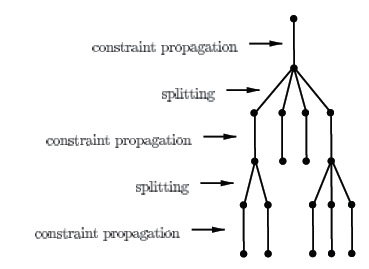
\includegraphics{tree.png}
\caption{Example of a CSP search tree. From Constraint Programming - lecture 3 (CSP) Algorithms. }
\label{fig:basic_tree}
\end{figure}

\subsection{The Backtracking Algorithm}

For creation and traversal of our Search Tree, we started with the backtracking algorithm as described in the assignment description.

\begin{verbatim}
procedure BT(X:variables, V:assignment, C:constraints)
    if X={} then return V
    x := select a not-yet assigned variable from X
    for each value h from the domain of x do
        if consistent(V+{x/h}, C) then
            R := BT(X-{x}, V+{x/h}, C)
        if R != fail then return R
    end for
    return fail
end BT
\end{verbatim}

In short, this algorithm takes a cell that is not yet assigned a value, and for each value in its domain creates a new branch in the search tree. The branches recursively create their own branches, forming a search tree. The tree is searched depth-first for a solution. The algorithm terminates if either a solution is found, or no solution exists in the search tree.

\subsection{Optimizations}

The Backtracking algorithm is, besides simple and effective, very inefficient. For each open cell in a Sudoku problem, the algorithm will create nine branches (one for each possible value). However, because we know the constraints, we can rule out complete branches of the search tree at early stages. There are also specific Sudoku solving techniques that help rule out possible values. Pruning the search tree with these methods way results in a smaller search space and therefore lower runtimes of the solver. In this section we describe the pruning methods we used, which correspond to the earlier-discussed constraint propogation.

\subsubsection{Revise / Constraint Propagation}

Also:
maintaining arc consistency (MAC)
. Now: local consistency notion is arcconsistency.
. Arc consistency binary constraints:
For every constraint C and every variable x with domain D, each
value for x from D participates in a solution to C
. Arc consistency:
En revise bekijkt ook arc consistency (i.e. constraints tussen 2 variables)


Our Revise method is a version of the AC-3 method as described in \citet{BartakConsistency}. It works as follows: When a value is assigned to a cell, because in a completed Sudoku each value should appear exactly once in each row, column and region, we can rule out the assigned value as a possibility for the other cells in its row, column and region. It is possible that this method implicitly creates a new assignment by ruling out a value from the domain of a cell with only two values left. Because of this, we apply the Revise method until no more changes are made. For efficiency, after the first revision, the Revise method only checks cells that could have been affected by the previous revision.

This method is capable of solving a Sudoku by itself without ever allowing the backtracking algorithm to branch, as we experienced with multiple Sudokus in the provided testset.

\subsubsection{Hidden Singles}



\subsubsection{Naked Pairs}

\subsubsection{Hidden Pairs}

\subsubsection{Heuristics}

From slides:
Complete labeling tree

ordering of variables does not differ in
number of leaves

ordering of variables does differ in number
of nodes

least number of nodes if the variables are
ordered by their domain sizes in the
increasing order

This is a bit like one of the heuristics with the lowest nr Children first stuff.

And later on:
Heuristics for search algorithms

Variable selection

Select a variable with the smallest domain

select a most constraint variable


select a variable with the smallest difference between its domain bounds

Heuristics for search algorithms

Value selection

select a value for which the heuristic function yields the hightest outcome

select the smallest value

select the largest value

select the middle value


\section{Implementation}

Java blabla

\section{Results}

Zoiets:

\begin{table}
\begin{center}
\begin{tabular}{c c c c c c}
\hline
 Revise & Hidden Singles & Hidden Pairs & Naked Pairs & sudoku\_training & top95 \\
\hline
x &  &  &  & 8m56s & 1h55m25s \\ % training_rv=536.094290474, top95_rv=6924.5242909
x & x & x & x & 25s & 10s \\ % training_rv_hs_hp_np_h13=25.511620738333335, top95_rv_hs_hp_np=9.685215524666667
x & x &  &  & 29s & 47s \\ % training_rv_hs=29.234435128, top95_rv_hs=47.415598335
x & x &  & x & 23s & 21s \\ % training_rv_hs_np=23.296235251333332,, top95_rv_hs_np=20.824697618666665
x & x & x &  & 28s & 16s \\ % training_rv_hs_hp=27.667227801666666,  top95_rv_hs_hp=15.692717729
x &   & x &  & 8m9s & 26m37s \\ % training_rv_hp=489.462033154, top95_rv_hp=1596.8818117199999
x &   & x & x & 1m21s & 3m51s \\ % training_rv_hp_np=81.19639021366667, top95_rv_hp_np=230.84322473
x &  &  & x & 1m17s & 19m32s \\ % training_rv_np=76.90551903866667, top95_rv_np=1172.4098914453334
\hline
\end{tabular}
\end{center}
\caption{The runtimes of our program using two different Sudoku sets with the different optimizations enabled (indicated with an x) or disabled. The times were averaged over three runs, except the revise-only trial which was only performed once.}
\end{table}

\begin{table}
\begin{center}
\begin{tabular}{c c c c c c}
\hline
 Revise & Heuristic 1 & Heuristic 3 & sudoku\_training & top95 \\
\hline
x &  &  & 8m56s & 1h55m25s \\ % training_rv=536.094290474, top95_rv=6924.5242909
x & x &  & 8m53s & 1h57m3s \\ % training_rv_h1=532.882686773, top95_rv_h1=7023.125097676
x &  & x & 9m3s & 1h57m40s \\ % training_rv_h3=543.003054551, top95_rv_h3=7060.009184544
x & x & x & 9m1s & 1h56m52s \\ % training_rv_h13=540.58733985, top95_rv_h13=7011.893442942
\hline
\end{tabular}
\end{center}
\caption{The runtimes of our program using two different Sudoku sets with only the revise algorithm and no, one or both heuristics enabled. These results are from a single run.}
\end{table}

% , , 

\begin{table}
\begin{center}
\begin{tabular}{c c c c c c}
\hline
 Revise & Hidden Singles & Heuristic 1 & Heuristic 3 & sudoku\_training & top95 \\
\hline
x & x &  &  & 29s & 47s \\ % training_rv_hs=29.234435128, top95_rv_hs=47.415598335
x & x & x &  & 29s & 50s \\ % training_rv_hs_h1=29.734570621, top95_rv_hs_h1=49.521653201
x & x &  & x & 30s & 48s \\ % training_rv_hs_h3=29.912008605, top95_rv_hs_h3=48.22889132033333
x & x & x & x & 29s & 52s \\ % training_rv_hs_h13=29.857984153, top95_rv_hs_h13=51.78545695633333
\hline
\end{tabular}
\end{center}
\caption{The runtimes of our program using two different Sudoku sets with only the revise algorithm and the hidden singles algorithm and no, one or both heuristics enabled. The times were averaged over three runs.}
\end{table}

\section{Conclusion}

\nocite{BartakConsistency}

\bibliographystyle{plainnat}
\bibliography{ref}

\end{document}
